% This file was created with tikzplotlib v0.10.1.
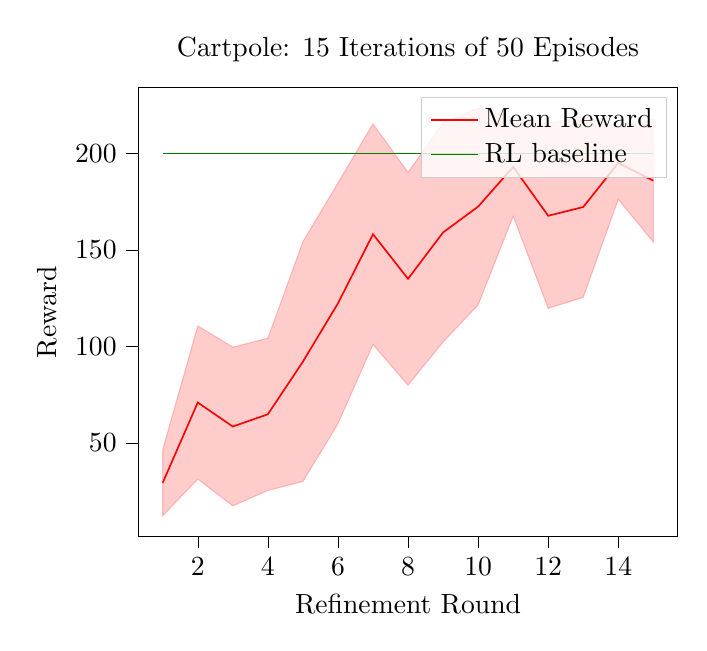
\begin{tikzpicture}

\definecolor{darkgray176}{RGB}{176,176,176}
\definecolor{green01270}{RGB}{0,127,0}
\definecolor{lightgray204}{RGB}{204,204,204}

\begin{axis}[
legend cell align={left},
legend style={fill opacity=0.8, draw opacity=1, text opacity=1, draw=lightgray204},
tick align=outside,
tick pos=left,
title={Cartpole: 15 Iterations of 50 Episodes},
x grid style={darkgray176},
xlabel={Refinement Round},
xmin=0.3, xmax=15.7,
xtick style={color=black},
y grid style={darkgray176},
ylabel={Reward},
ymin=1.62542024959169, ymax=233.917770642266,
ytick style={color=black}
]
\path [draw=red, fill=red, opacity=0.2]
(axis cs:1,46.5118365507413)
--(axis cs:1,12.1841634492587)
--(axis cs:2,31.1995030609939)
--(axis cs:3,17.3279571466358)
--(axis cs:4,25.3223243632786)
--(axis cs:5,29.9457090472551)
--(axis cs:6,59.8716286122037)
--(axis cs:7,100.912690545278)
--(axis cs:8,79.8388788988171)
--(axis cs:9,102.232611965941)
--(axis cs:10,121.416972557401)
--(axis cs:11,167.392068044626)
--(axis cs:12,119.668304864884)
--(axis cs:13,125.369028357119)
--(axis cs:14,176.179632759657)
--(axis cs:15,154.017086592502)
--(axis cs:15,217.622913407498)
--(axis cs:15,217.622913407498)
--(axis cs:14,213.860367240343)
--(axis cs:13,218.982971642881)
--(axis cs:12,215.611695135116)
--(axis cs:11,218.559931955374)
--(axis cs:10,223.359027442599)
--(axis cs:9,215.799388034059)
--(axis cs:8,190.137121101183)
--(axis cs:7,215.271309454722)
--(axis cs:6,184.688371387796)
--(axis cs:5,154.174290952745)
--(axis cs:4,104.269675636721)
--(axis cs:3,99.5600428533642)
--(axis cs:2,110.584496939006)
--(axis cs:1,46.5118365507413)
--cycle;

\addplot [semithick, red]
table {%
1 29.348
2 70.892
3 58.444
4 64.796
5 92.06
6 122.28
7 158.092
8 134.988
9 159.016
10 172.388
11 192.976
12 167.64
13 172.176
14 195.02
15 185.82
};
\addlegendentry{Mean Reward}
\addplot [semithick, green01270]
table {%
1 200
2 200
3 200
4 200
5 200
6 200
7 200
8 200
9 200
10 200
11 200
12 200
13 200
14 200
15 200
};
\addlegendentry{RL baseline}
\end{axis}

\end{tikzpicture}
